\documentclass[aspectratio=169,11pt]{beamer}

\usetheme{Madrid}
\usecolortheme{seahorse}
\usepackage{booktabs}
\usepackage{graphicx}

\title[Token pruning]{Inference-Time Token Pruning}
\subtitle{Person re-identification is the evaluation task}
\author[Nazmul Hasan Nazim]{Nazmul Hasan Nazim\\Student ID 2527369}
\institute[CSE553.1]{CSE553.1 Computer Vision\\Course faculty: Dr.\ Nabeel Mohammed (NbM)}
\date{}
\setbeamertemplate{navigation symbols}{}

\begin{document}

\begin{frame}
\titlepage
\end{frame}

\begin{frame}{The question}
A frozen vision transformer normally keeps every patch token through all 12 blocks.
\begin{itemize}
\item Can later blocks run after some patch tokens are dropped?
\item Does the choice of patches matter?
\item Does a shorter sequence have a measured latency benefit?
\end{itemize}
\vspace{0.7em}
Person re-identification is how that question is scored.\\
One crop is used to rank other photographs of the same person.
\end{frame}

\begin{frame}{What a visual token is}
\begin{itemize}
\item The image is $256 \times 128$.
\item Patch size 16 gives a $16 \times 8$ grid: 128 patch tokens.
\item One class token is added. The sequence length is 129.
\item The class token mixes with the patches in every block.
\item The search vector is built from the class token: 1{,}280 dimensions, then cosine.
\end{itemize}
\vspace{0.5em}
A patch token is one cell of that grid, not a detected object.
\end{frame}

\begin{frame}{Where pruning happens}
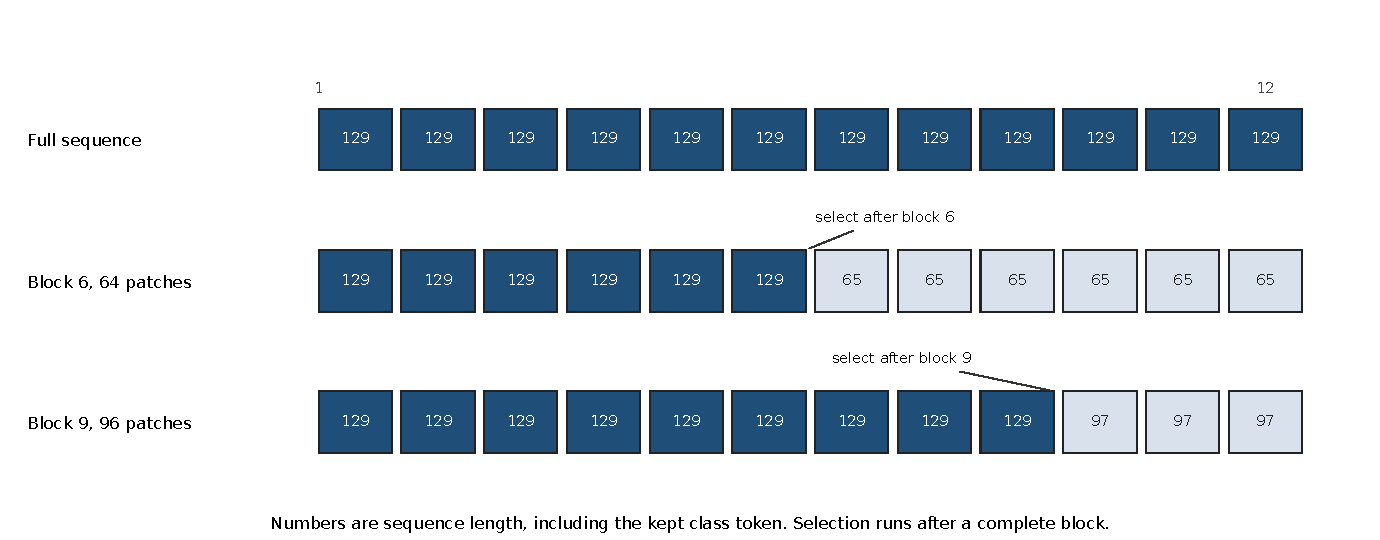
\includegraphics[width=0.98\linewidth]{figures/token_flow.pdf}
\vspace{0.3em}

\footnotesize
Selection runs after a complete block. The class token is kept.\\
Block 6 with 64 patches: blocks 7--12 see 65 tokens.\\
Block 9 with 96 patches: blocks 10--12 see 97 tokens.
\end{frame}

\begin{frame}{Two ways to choose the same number of patches}
\begin{columns}[T]
\begin{column}{0.48\textwidth}
\textbf{Class attention}\\[0.4em]
Keep the patches with the highest class-token attention.\\
Accuracy tables use the reference scores.\\
The extra attention call stays inside the measured time.
\end{column}
\begin{column}{0.48\textwidth}
\textbf{Random control}\\[0.4em]
Draw the same count uniformly.\\
Five seeds: 11, 23, 37, 53, 71.\\
The draw does not use the identity.
\end{column}
\end{columns}
\vspace{0.8em}
These two cuts change depth and patch count together.\\
They do not isolate one of those choices by itself.\\[0.4em]
Block 9 / 96 was fixed on a training-identity split before the official test.\\
That split is identity-seen. Its high scores are not this result.
\end{frame}

\begin{frame}{How a score is read}
The encoder is a published CLIP-ReID checkpoint. It is frozen.
\begin{itemize}
\item Rank-1: the first allowed gallery photo is the right person.
\item mAP: the whole list of true matches is in good order.
\item Official test: 3{,}368 queries, 15{,}913 gallery images, 750 people who were not in training.
\end{itemize}
\vspace{0.5em}
This checkpoint scores 89.41\% mAP and 94.98\% Rank-1.\\
The published Rank-1 is 95.5. The gap is 0.52 percentage points.\\
That is an approximate reproduction.
\end{frame}

\begin{frame}{Official test}
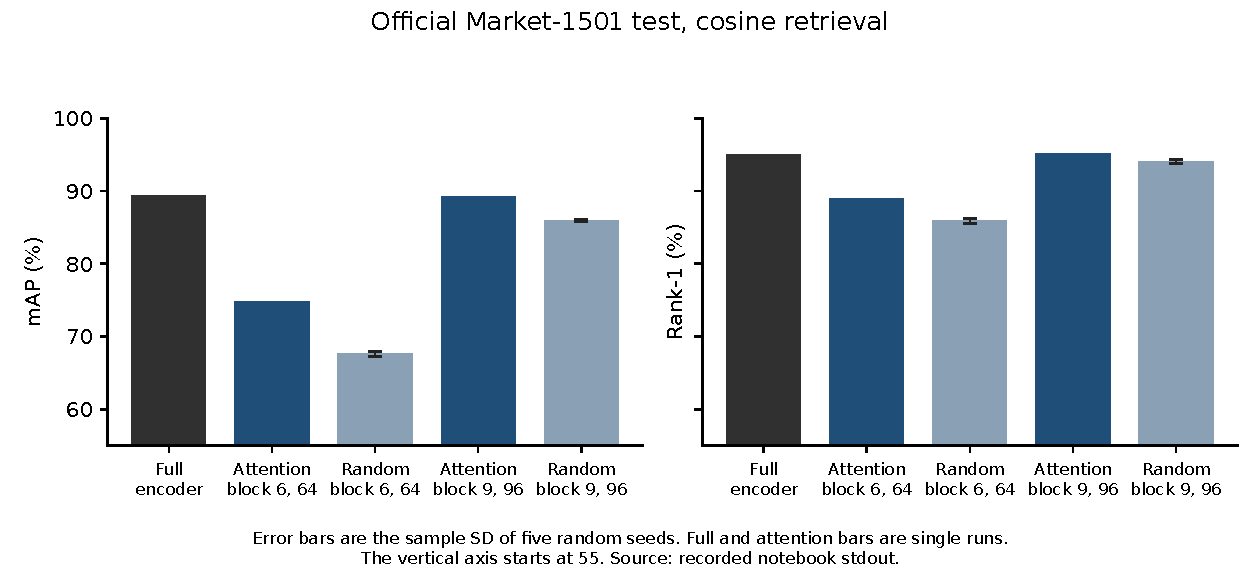
\includegraphics[width=0.92\linewidth]{figures/official_test_accuracy.pdf}
\vspace{0.2em}

\footnotesize
Cosine retrieval. Error bars are the five-seed sample standard deviation.\\
Full and attention bars are single runs.
\end{frame}

\begin{frame}{Attention against the random control}
From the unrounded scores, sample standard deviation across five seeds:
\begin{center}
\small
\begin{tabular}{lcc}
\toprule
Official test & mAP & Rank-1 \\
\midrule
Full encoder & 89.41 & 94.98 \\
Attention, block 6, 64 patches & 74.86 & 88.93 \\
Random, block 6, 64 & 67.63 $\pm$ 0.33 & 85.89 $\pm$ 0.30 \\
Attention, block 9, 96 patches & 89.27 & 95.13 \\
Random, block 9, 96 & 85.97 $\pm$ 0.12 & 94.07 $\pm$ 0.22 \\
\bottomrule
\end{tabular}
\end{center}
\vspace{0.3em}
\footnotesize
Attention is above its matched random mean at both cuts.\\
Block 6 / 64 costs 14.55 mAP percentage points against the full encoder.\\
Block 9 / 96 does not establish a better accuracy--cost operating point.
\end{frame}

\begin{frame}{One query}
\begin{columns}[c]
\begin{column}{0.40\textwidth}
\centering

\includegraphics[height=0.68\textheight]{figures/0001_c1s1_001051_00_keep50.png}
\end{column}
\begin{column}{0.56\textwidth}
Real Market-1501 query \texttt{0001}.\\[0.5em]
Dark blocks were dropped after block 6.\\
64 of 128 patches stayed.\\[0.5em]
By that block the class token and the patch tokens have already mixed.\\[0.5em]
A dark block is not proof that only background was removed.\\
The picture is one query.
\end{column}
\end{columns}
\end{frame}

\begin{frame}{Measured time, block 6 / 64 only}
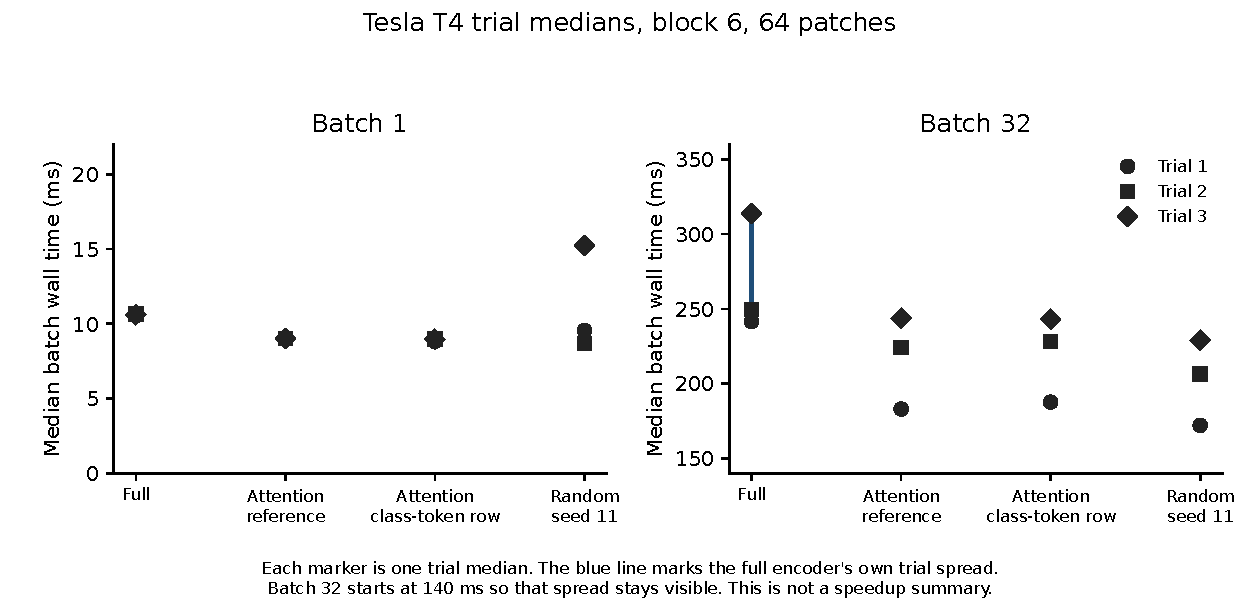
\includegraphics[width=0.78\linewidth]{figures/timing_trials.pdf}
\vspace{0.15em}

\footnotesize
Batch-32 full-encoder medians: 241.5, 249.6, and 313.7\,ms.\\
That spread is why the ratios are not an established speedup.\\
Block 9 / 96 was not timed. Fewer tokens are not, by themselves, a latency result.
\end{frame}

\begin{frame}{What the measurement supports}
\begin{itemize}
\item The selection rule is the class-attention rule from EViT, used once, without its training or token fusion.
\item The contribution is the measurement on this frozen re-identification encoder.
\item Dropping 64 patches after block 6 costs 14.55 percentage points of mAP.
\item Keeping 96 patches after block 9 stays close to the full encoder on this test.
\item Class attention beats the five-seed random mean at the same patch count.
\item The timings do not establish a speedup.
\end{itemize}
\end{frame}

\begin{frame}{References}
\begin{itemize}
\item Zheng et al., Market-1501, ICCV 2015.
\item Li, Sun, and Li, CLIP-ReID, AAAI 2023.
\item Dosovitskiy et al., Vision Transformer, ICLR 2021.
\item Liang et al., EViT, ICLR 2022.
\item Zhong et al., k-reciprocal re-ranking, CVPR 2017.
\item Radford et al., CLIP, ICML 2021.
\end{itemize}
\vspace{0.6em}
\footnotesize
Code that produced the numbers: \texttt{d143dbd}.\\
Paper record checked at \texttt{24e36ac}. Full-validation stdout saved in \texttt{c2a5246}.
\end{frame}

\end{document}
